
\subsection{Glyph: \glyph{Simple chemical}}
\label{sec:simpleChemical}

In SBGN \PDs, a simple chemical is defined as the opposite of a macromolecule (\sect{macromolecule}): it is a chemical compound that is \emph{not} formed by the covalent linking of pseudo-identical residues.  Examples of simple chemicals are an atom, a monoatomic ion, a salt, a radical, a solid metal, a crystal, etc. A \glyph{simple chemical} is represented by a circular
container, as depicted in \fig{simpleChemical}. To avoid confusion with the Unspecified Entity (\ref{sec:unspecifiedEntity}), this glyph must remain a circle and cannot be deformed into an eclipse.

\begin{figure}[H]
  \centering
  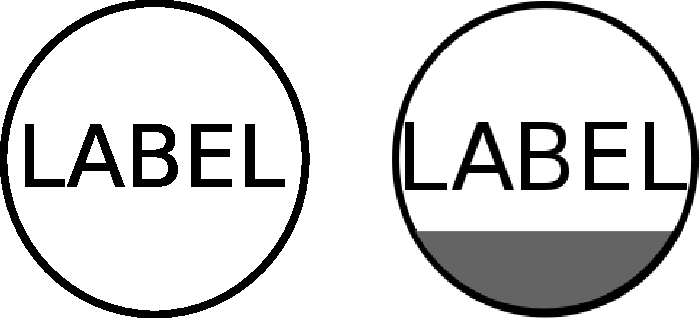
\includegraphics[scale = 0.3]{images/simpleChemical}
  \caption{The \PD glyph for \glyph{simple chemical}.}
  \label{fig:simpleChemical}
\end{figure}
